%%%%%%%%%%%%%%%%%%%%%%%%%%%%%%%%%%%%%%%%%
% Beamer Presentation
% LaTeX Template
% Version 2.0 (March 8, 2022)
%
% This template originates from:
% https://www.LaTeXTemplates.com
%
% Author:
% Vel (vel@latextemplates.com)
%
% License:
% CC BY-NC-SA 4.0 (https://creativecommons.org/licenses/by-nc-sa/4.0/)
%
%%%%%%%%%%%%%%%%%%%%%%%%%%%%%%%%%%%%%%%%%

%----------------------------------------------------------------------------------------
%	PACKAGES AND OTHER DOCUMENT CONFIGURATIONS
%----------------------------------------------------------------------------------------

\documentclass[
	11pt, % Set the default font size, options include: 8pt, 9pt, 10pt, 11pt, 12pt, 14pt, 17pt, 20pt
	%t, % Uncomment to vertically align all slide content to the top of the slide, rather than the default centered
	%aspectratio=169, % Uncomment to set the aspect ratio to a 16:9 ratio which matches the aspect ratio of 1080p and 4K screens and projectors
]{beamer}

\graphicspath{{Images/}{./}} % Specifies where to look for included images (trailing slash required)

\usepackage{booktabs} % Allows the use of \toprule, \midrule and \bottomrule for better rules in tables
\usepackage{wrapfig}
\usepackage{listings}
\usepackage{adjustbox}

%----------------------------------------------------------------------------------------
%	SELECT LAYOUT THEME
%----------------------------------------------------------------------------------------

% Beamer comes with a number of default layout themes which change the colors and layouts of slides. Below is a list of all themes available, uncomment each in turn to see what they look like.

%\usetheme{default}
%\usetheme{AnnArbor}
%\usetheme{Antibes}
%\usetheme{Bergen}
%\usetheme{Berkeley}
%\usetheme{Berlin}
%\usetheme{Boadilla}
%\usetheme{CambridgeUS}
%\usetheme{Copenhagen}
\usetheme{Darmstadt}
%\usetheme{Dresden}
%\usetheme{Frankfurt}
%\usetheme{Goettingen}
%\usetheme{Hannover}
%\usetheme{Ilmenau}
%\usetheme{JuanLesPins}
%\usetheme{Luebeck}
%\usetheme{Madrid}
%\usetheme{Malmoe}
%\usetheme{Marburg}
%\usetheme{Montpellier}
%\usetheme{PaloAlto}
%\usetheme{Pittsburgh}
%\usetheme{Rochester}
%\usetheme{Singapore}
%\usetheme{Szeged}
%\usetheme{Warsaw}

%----------------------------------------------------------------------------------------
%	SELECT COLOR THEME
%----------------------------------------------------------------------------------------

% Beamer comes with a number of color themes that can be applied to any layout theme to change its colors. Uncomment each of these in turn to see how they change the colors of your selected layout theme.

%\usecolortheme{albatross}
%\usecolortheme{beaver}
%\usecolortheme{beetle}
%\usecolortheme{crane}
%\usecolortheme{dolphin}
%\usecolortheme{dove}
%\usecolortheme{fly}
\usecolortheme{lily}
%\usecolortheme{monarca}
%\usecolortheme{seagull}
%\usecolortheme{seahorse}
%\usecolortheme{spruce}
%\usecolortheme{whale}
%\usecolortheme{wolverine}

%----------------------------------------------------------------------------------------
%	SELECT FONT THEME & FONTS
%----------------------------------------------------------------------------------------

% Beamer comes with several font themes to easily change the fonts used in various parts of the presentation. Review the comments beside each one to decide if you would like to use it. Note that additional options can be specified for several of these font themes, consult the beamer documentation for more information.

\usefonttheme{default} % Typeset using the default sans serif font
%\usefonttheme{serif} % Typeset using the default serif font (make sure a sans font isn't being set as the default font if you use this option!)
%\usefonttheme{structurebold} % Typeset important structure text (titles, headlines, footlines, sidebar, etc) in bold
%\usefonttheme{structureitalicserif} % Typeset important structure text (titles, headlines, footlines, sidebar, etc) in italic serif
%\usefonttheme{structuresmallcapsserif} % Typeset important structure text (titles, headlines, footlines, sidebar, etc) in small caps serif

%------------------------------------------------

%\usepackage{mathptmx} % Use the Times font for serif text
\usepackage{palatino} % Use the Palatino font for serif text

%\usepackage{helvet} % Use the Helvetica font for sans serif text
\usepackage[default]{opensans} % Use the Open Sans font for sans serif text
%\usepackage[default]{FiraSans} % Use the Fira Sans font for sans serif text
%\usepackage[default]{lato} % Use the Lato font for sans serif text

%----------------------------------------------------------------------------------------
%	SELECT INNER THEME
%----------------------------------------------------------------------------------------

% Inner themes change the styling of internal slide elements, for example: bullet points, blocks, bibliography entries, title pages, theorems, etc. Uncomment each theme in turn to see what changes it makes to your presentation.

%\useinnertheme{default}
\useinnertheme{circles}
%\useinnertheme{rectangles}
%\useinnertheme{rounded}
%\useinnertheme{inmargin}

%----------------------------------------------------------------------------------------
%	SELECT OUTER THEME
%----------------------------------------------------------------------------------------

% Outer themes change the overall layout of slides, such as: header and footer lines, sidebars and slide titles. Uncomment each theme in turn to see what changes it makes to your presentation.

%\useoutertheme{default}
%\useoutertheme{infolines}
%\useoutertheme{miniframes}
%\useoutertheme{smoothbars}
%\useoutertheme{sidebar}
%\useoutertheme{split}
%\useoutertheme{shadow}
%\useoutertheme{tree}
%\useoutertheme{smoothtree}

%\setbeamertemplate{footline} % Uncomment this line to remove the footer line in all slides
%\setbeamertemplate{footline}[page number] % Uncomment this line to replace the footer line in all slides with a simple slide count

\setbeamertemplate{navigation symbols}{} % Uncomment this line to remove the navigation symbols from the bottom of all slides

%----------------------------------------------------------------------------------------
%	PRESENTATION INFORMATION
%----------------------------------------------------------------------------------------

\title[Ansible]{Ansible} % The short title in the optional parameter appears at the bottom of every slide, the full title in the main parameter is only on the title page

\subtitle{Automation platform} % Presentation subtitle, remove this command if a subtitle isn't required

\author[Lucía Martín Serrano]{Lucía Martín Serrano} % Presenter name(s), the optional parameter can contain a shortened version to appear on the bottom of every slide, while the main parameter will appear on the title slide

\institute[UCLM]{Universidad de Castilla-La Mancha \\ \smallskip \textit{Lucia.Martin17@alu.uclm.es}} % Your institution, the optional parameter can be used for the institution shorthand and will appear on the bottom of every slide after author names, while the required parameter is used on the title slide and can include your email address or additional information on separate lines

%\date[\today]{International Symposium of Explorers \\ \today} % Presentation date or conference/meeting name, the optional parameter can contain a shortened version to appear on the bottom of every slide, while the required parameter value is output to the title slide

%----------------------------------------------------------------------------------------

\begin{document}

%----------------------------------------------------------------------------------------
%	TITLE SLIDE
%----------------------------------------------------------------------------------------

\begin{frame}
	\titlepage % Output the title slide, automatically created using the text entered in the PRESENTATION INFORMATION block above
\end{frame}

%----------------------------------------------------------------------------------------
%	TABLE OF CONTENTS SLIDE
%----------------------------------------------------------------------------------------

% The table of contents outputs the sections and subsections that appear in your presentation, specified with the standard \section and \subsection commands. You may either display all sections and subsections on one slide with \tableofcontents, or display each section at a time on subsequent slides with \tableofcontents[pausesections]. The latter is useful if you want to step through each section and mention what you will discuss.

\begin{frame}
	\frametitle{Sipnosis de la presentación} % Slide title, remove this command for no title
	
	\tableofcontents % Output the table of contents (all sections on one slide)
	%\tableofcontents[pausesections] % Output the table of contents (break sections up across separate slides)
\end{frame}

%----------------------------------------------------------------------------------------
%	PRESENTATION BODY SLIDES
%----------------------------------------------------------------------------------------

\section{Introducción} % Sections are added in order to organize your presentation into discrete blocks, all sections and subsections are automatically output to the table of contents as an overview of the talk but NOT output in the presentation as separate slides

%------------------------------------------------

\begin{frame}
	\frametitle{Introducción (I)}

    \begin{itemize}
        \item La \textbf{automatización} es el uso de la tecnología para realizar tareas con la menor presencia humana posible.
        \item Cualquier industria que conlleve tareas repetitivas puede usar la automatización, y en este caso tareas como el \textbf{aprovisionamiento}, \textbf{configuración de la red} o la \textbf{gestión de la configuración} pueden ser automatizadas. \cite{p1}
        
    \end{itemize}

\end{frame}

%------------------------------------------------

\begin{frame}
	\frametitle{Introducción (II)}

        \begin{block}{Aprovisionamiento}
            El \textbf{aprovisionamiento} tiene que ver con el trabajo pesado, ya sea en hardware dedicado o en una nube privada, híbrida o pública.\\
            Para ejecutar sistemas empresariales, se necesita infraestructura y esa infraestructura debe estar \textbf{configurada}.
        \end{block}
        \begin{block}{}
            Lo que antes se trataba de racks, cajas y cables en un centro de datos, ahora (en su mayoría) se trata de activos virtualizados, desde centros de datos definidos por software, redes y almacenamiento hasta máquinas virtuales y contenedores. \cite{p1}
        \end{block}

\end{frame}

%------------------------------------------------

\begin{frame}
	\frametitle{Introducción (III)}

        \begin{block}{Gestión de la configuración}
            No todas las aplicaciones se crean de la misma manera. Requieren diferentes configuraciones, sistemas de archivos, puertos, usuarios... y la lista continúa. Una vez que haya automatizado el aprovisionamiento, debe poder indicar a esos recursos lo que deben hacer.
        \end{block}
        \begin{block}{}
            Para ello, necesita una solución de \textbf{gestión de la configuración} sólida que permita a los desarrolladores definir simplemente la infraestructura de forma que todos los miembros de su equipo de TI puedan entenderla fácilmente. Cuanto más sencillo sea \textbf{automatizar los scripts y las prácticas ad hoc} para la gestión del sistema, más fácil será realizar el trabajo real. \cite{p1}
        \end{block}

\end{frame}

%------------------------------------------------

\section{¿Qué es Ansible?}

\subsection{Historia de Ansible}

\begin{frame}
	\frametitle{Historia de Ansible (I)}
	
	\begin{itemize}
		\item El término "ansible" fue acuñado por Ursula K. Le Guin en su novela de 1966 Rocannon's World, y se refiere a los sistemas ficticios de comunicación instantánea.

            \item La herramienta Ansible fue desarrollada por \textbf{Michael DeHaan}, autor de la aplicación de servidor de aprovisionamiento Cobbler y coautor del marco Fedora Unified Network Controller (Func) para la administración remota. \cite{p2}
		
	\end{itemize}
	
\end{frame}

%------------------------------------------------

\begin{frame}
	\frametitle{Historia de Ansible (II)}
	
	\begin{block}{Ansible, Inc.}
		\textbf{Ansible, Inc.} (originalmente AnsibleWorks, Inc.) fue la empresa fundada en 2013 por DeHaan, Timothy Gerla y Saïd Ziouani para apoyar y patrocinar comercialmente a Ansible.  \textbf{Red Hat} adquirió Ansible en octubre de 2015.

	\end{block}
        \begin{block}{Compatibilidad}
            Ansible se incluye como parte de la distribución Fedora de Linux, propiedad de Red Hat, y también está disponible para Red Hat Enterprise Linux, CentOS, openSUSE, SUSE Linux Enterprise, Debian, Ubuntu, Scientific Linux y Oracle Linux a través de paquetes adicionales para Enterprise Linux, así como para otros sistemas operativos. \cite{p2}
        \end{block}
	
\end{frame}

%------------------------------------------------

\begin{frame}
	\frametitle{Historia de Ansible (III)}

        \begin{figure}
		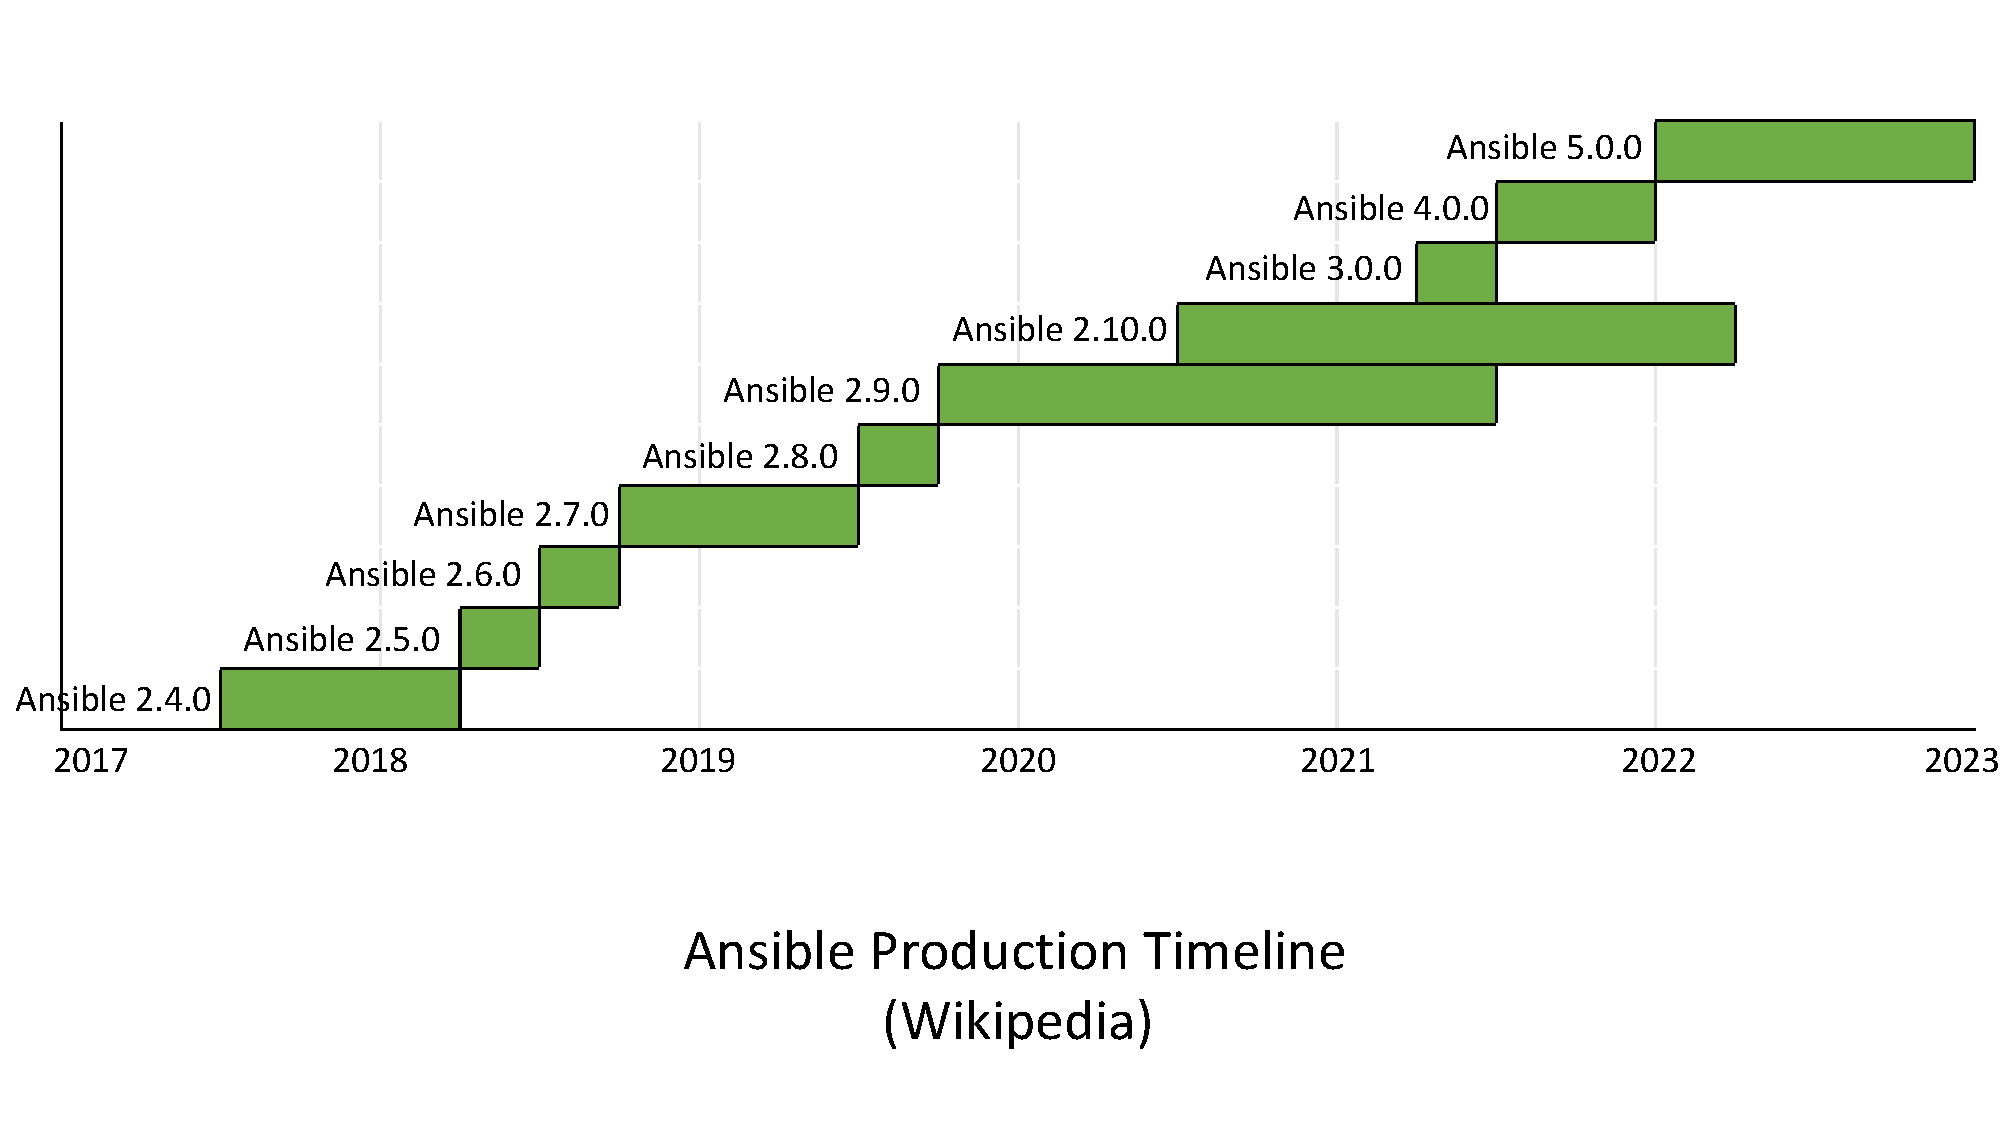
\includegraphics[width=1.0\linewidth]{timeline.pdf}
            \caption{Línea del tiempo de producción de Ansible}
	\end{figure}
	
\end{frame}

%------------------------------------------------

\subsection{Definición}

\begin{frame}
	\frametitle{Ansible, Plataforma de automatización}

    \begin{wrapfigure}{r}{0.5\textwidth}
        \centering
        
\includegraphics[width=0.5\linewidth]{ansible_logo.pdf}
        \label{fig:ansible-logo}
    \end{wrapfigure}
    
    \textbf{Ansible} es una herramienta software de automatización de TI de código abierto que que reduce la complejidad y se ejecuta en todas partes. El uso de Ansible permite automatizar prácticamente cualquier tarea.

\end{frame}

%------------------------------------------------

\begin{frame}
	\frametitle{Características}

        \begin{exampleblock}{Casos de Uso}
        Con Ansible puedes:
		\begin{itemize}
		    \item Eliminar la repetición y simplificar los flujos de trabajo
                \item Administrar y mantiener la configuración del sistema
                \item Implementar continuamente software complejo
                \item Realizar actualizaciones continuas sin tiempo de inactividad
		\end{itemize}
	\end{exampleblock}

        \begin{exampleblock}{Princípios}
		\begin{itemize}
		    \item Arquitectura sin agentes
                \item Simplicidad
                \item Escalabilidad y flexibilidad
                \item Idempotencia y previsibilidad
		\end{itemize}
	\end{exampleblock}

\end{frame}

%------------------------------------------------

\section{¿Cómo funciona?}

\begin{frame}
	\frametitle{Blocks of Highlighted Text}
	
	\begin{block}{Block Title}
		Lorem ipsum dolor sit amet, consectetur adipiscing elit. Integer lectus nisl, ultricies in feugiat rutrum, porttitor sit amet augue.
	\end{block}
	
	\begin{exampleblock}{Example Block Title}
		Aliquam ut tortor mauris. Sed volutpat ante purus, quis accumsan.
	\end{exampleblock}
	
	\begin{alertblock}{Alert Block Title}
		Pellentesque sed tellus purus. Class aptent taciti sociosqu ad litora torquent per conubia nostra, per inceptos himenaeos.
	\end{alertblock}

\end{frame}

%------------------------------------------------

\begin{frame}
	\frametitle{Multiple Columns}
	\framesubtitle{Subtitle} % Optional subtitle
	
	\begin{columns}[c] % The "c" option specifies centered vertical alignment while the "t" option is used for top vertical alignment
		\begin{column}{0.45\textwidth} % Left column width
			\textbf{Heading}
			\begin{enumerate}
				\item Statement
				\item Explanation
				\item Example
			\end{enumerate}
		\end{column}
		\begin{column}{0.5\textwidth} % Right column width
			Lorem ipsum dolor sit amet, consectetur adipiscing elit. Integer lectus nisl, ultricies in feugiat rutrum, porttitor sit amet augue. Aliquam ut tortor mauris. Sed volutpat ante purus, quis accumsan dolor.
		\end{column}
	\end{columns}
\end{frame}

%------------------------------------------------
\section{Alternativas}

\begin{frame}
	\frametitle{Ansible vs. Terraform vs. Puppet vs. Chef vs. Saltstack}
	
	\begin{figure}
		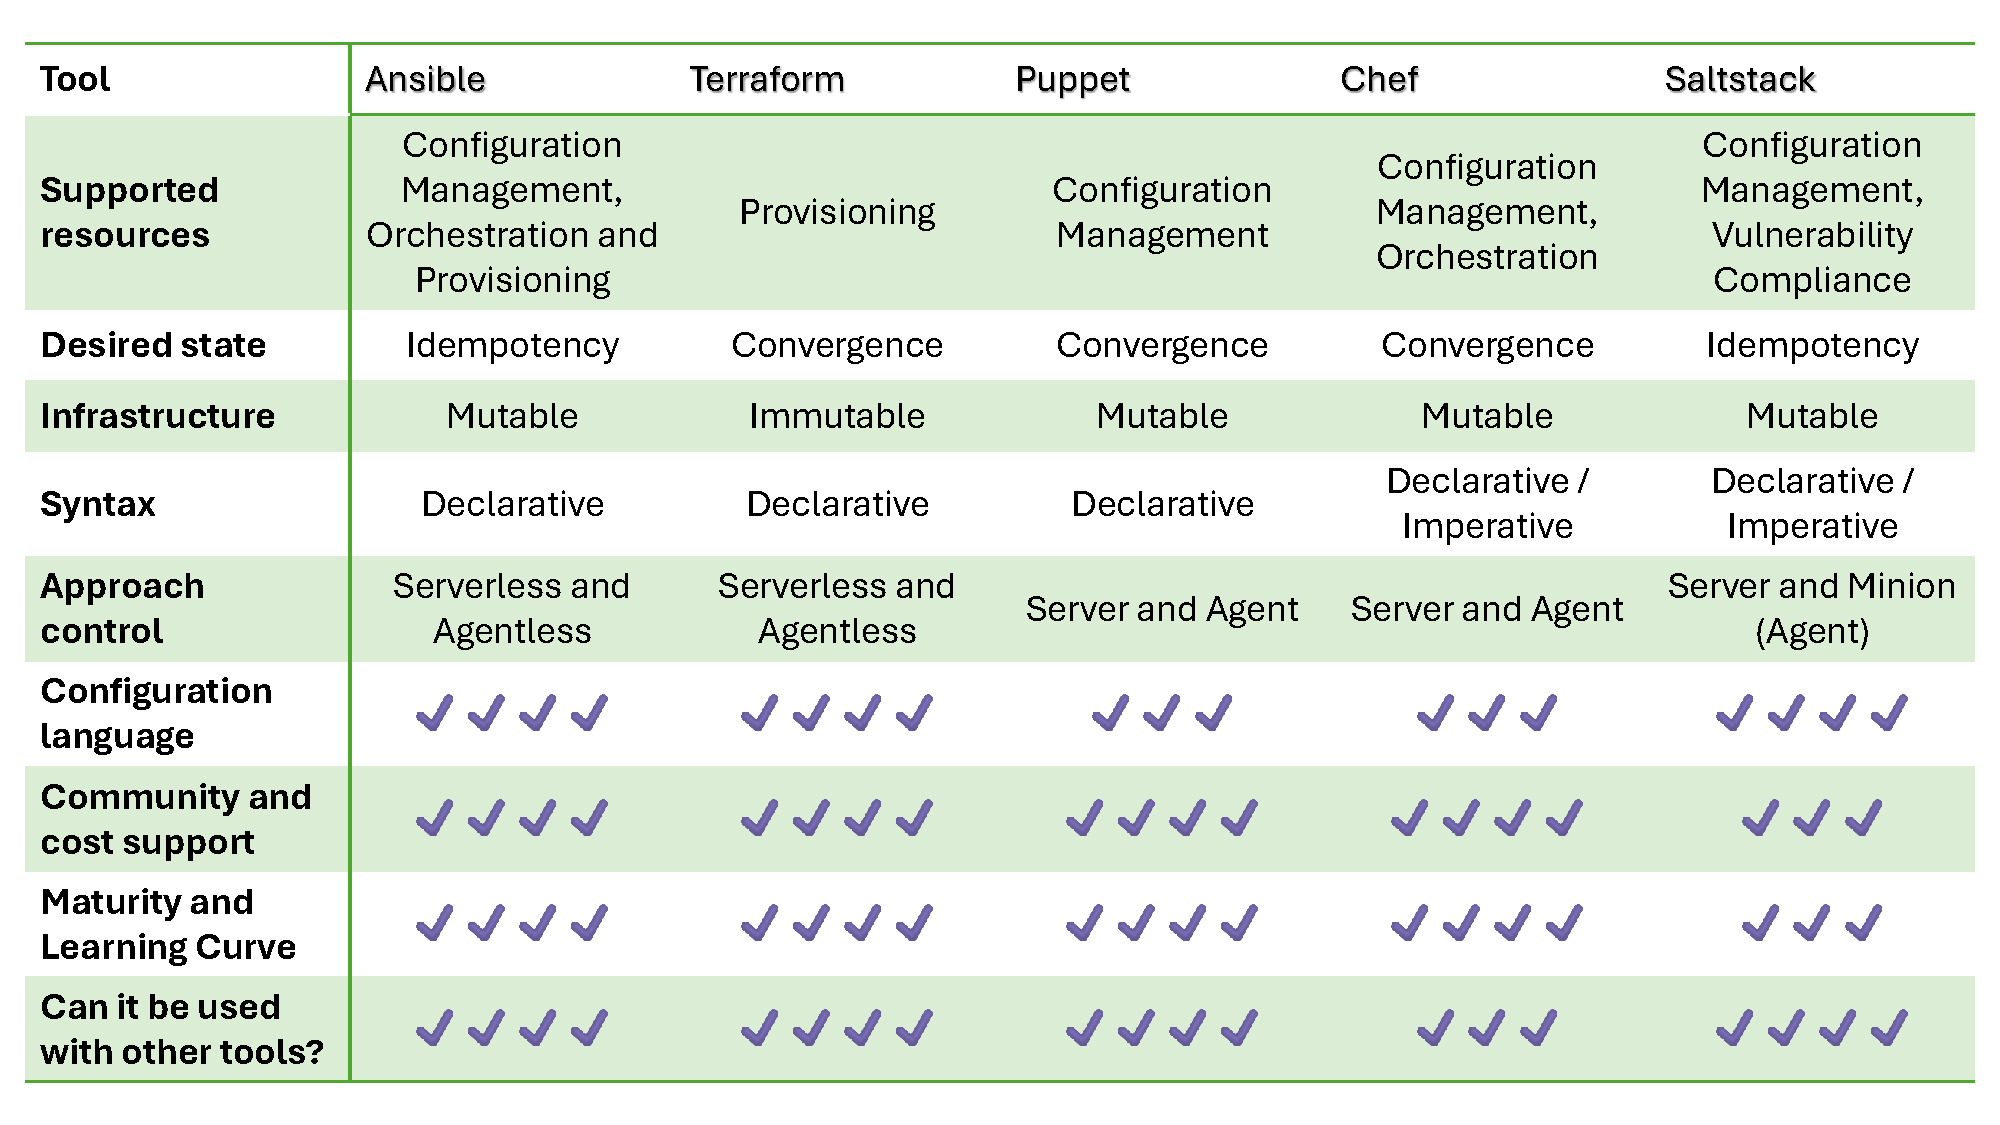
\includegraphics[width=0.9\linewidth]{alternativaTabla.pdf}
            \caption{Tabla comparativa \href{https://coralogix.com/blog/the-definitive-guide-to-configuration-management-tools/}{\cite{p5}}}
	\end{figure}

\end{frame}

%------------------------------------------------

\section{Demo}

\begin{frame}
	\frametitle{Demo}
	
\end{frame}

%------------------------------------------------

\section{Bibliografía}

\begin{frame} % Use [allowframebreaks] to allow automatic splitting across slides if the content is too long
	\frametitle{Referencias (I)}
	
	\begin{thebibliography}{99} % Beamer does not support BibTeX so references must be inserted manually as below, you may need to use multiple columns and/or reduce the font size further if you have many references
		\footnotesize % Reduce the font size in the bibliography
		
		\bibitem[Red Hat, 2023]{p1}
                Red Hat (2023)
                \newblock Understanding Automation
                \newblock \emph{www.redhat.com}. Disponible en: \url{https://www.redhat.com/en/topics/automation}
   
            \bibitem[Wikipedia, 2024]{p2}
                Wikipedia (2024)
                \newblock Ansible (software)
                \newblock \emph{en.wikipedia.org}. Disponible en: \url{https://en.wikipedia.org/wiki/Ansible\_\%28software\%29}
            
			\bibitem[docs-ansible, 2024]{p3}
                Ansible (2024)
                \newblock Introduction to Ansible-Ansible documentation
                \newblock \emph{docs.ansible.com}. Disponible en: \url{https://docs.ansible.com/ansible/latest/getting_started/introduction.html}

	\end{thebibliography}
\end{frame}

%------------------------------------------------

\begin{frame} % Use [allowframebreaks] to allow automatic splitting across slides if the content is too long
	\frametitle{Referencias (II)}
	
	\begin{thebibliography}{99} % Beamer does not support BibTeX so references must be inserted manually as below, you may need to use multiple columns and/or reduce the font size further if you have many references
		\footnotesize % Reduce the font size in the bibliography
		
		\bibitem[DigitalOcean, 2020]{p4}
				DigitalOcean (2020)
                \newblock {A}n {I}ntroduction to {C}onfiguration {M}anagement with {A}nsible
                \newblock \emph{www.digitalocean.com}. Disponible en: \url{https://www.digitalocean.com/community/conceptual-articles/an-introduction-to-configuration-management-with-ansible}
   
            \bibitem[Coralogix, 2020]{p5}
                Coralogix (2020)
                \newblock The Definitive Guide to Configuration Management Tools
                \newblock \emph{coralogix.com}. Disponible en: \url{https://coralogix.com/blog/the-definitive-guide-to-configuration-management-tools/}
            
			\bibitem[docs-ansible, 2024]{p6}
                Ansible (2024)
                \newblock Introduction to Ansible-Ansible documentation
                \newblock \emph{docs.ansible.com}. Disponible en: \url{https://docs.ansible.com/ansible/latest/getting_started/introduction.html}

	\end{thebibliography}
\end{frame}

%----------------------------------------------------------------------------------------
%	CLOSING SLIDE
%----------------------------------------------------------------------------------------

\section{¿Preguntas?}

\begin{frame}[plain]
	\begin{center}
		{\Huge \textcolor{blue}{Fin}}
		
		\bigskip\bigskip
		
		{\LARGE \textcolor{gray}{¿Preguntas? ¿Comentarios?}}
	\end{center}
\end{frame}

%----------------------------------------------------------------------------------------

\end{document} 